\chapter{Principe des actions réciproques}
\section{Source et cible}
Lorsque la notion de force a été définie en début de chapitre, elle a été présentée comme caractérisant \enquote{l'interaction} entre deux corps. Une force décrit toujours l'action exercée par un corps sur un autre et il n'existe pas de force sans qu'au moins deux ne soient concernés.
%Il n'existe pas de situation dans laquelle une force s'exerce sur un corps sans que celle-ci ne soit l'action d'un deuxième corps. 
%un corps agit sur un autre sans que ce deuxième n'agisse en retour sur le premier.

Afin d'éviter les confusions, il sera important de préciser le corps qui exerce la force -- la \motcle{source} -- et celui sur lequel s'exerce la force -- la \motcle{cible} -- .

\section{Mise en situation}
Une personne se tient debout, face à un mur sur lequel elle pousse.

\begin{tabular}{m{.3\linewidth} m{.7\linewidth}}
    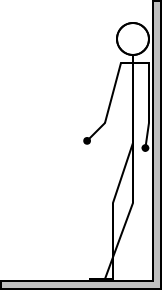
\includegraphics[width=.75 \linewidth]{actions_reciproques_1.png}
    %\label{Une personne appuyee contre un mur.}
    %\caption{actions_reciproques_1}
     &
    \begin{itemize}
        \item Quelle est la source de la force ?
              \pointilles{1}
        \item Quel est le corps cible ?
              \pointilles{1}
        \item Représente cette force sur le schéma.
    \end{itemize}
\end{tabular}

\newpage

Si, dans la même situation, la personne se tient sur une planche à roulettes.

\begin{tabular}{m{.3\linewidth} m{.7\linewidth}}
    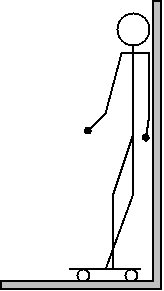
\includegraphics[width=.75 \linewidth]{actions_reciproques_2.png}
    %\label{Une personne appuyee contre un mur.}
    %\caption{actions_reciproques_1}
     &
    \begin{itemize}
        \item Que se passe-t-il lorsqu'elle s'appuie contre le mur ?
              \pointilles{2}
        \item Que peux-tu en conclure ?
              \pointilles{3}
    \end{itemize}
\end{tabular}

\begin{itemize}
    \item Quelle est la cible de cette nouvelle force ?
          \pointilles{1}
    \item Quel est le corps source ?
          \pointilles{1}
    \item Quel est le sens de cette force ?
    \item Représente cette force sur le schéma.
\end{itemize}

Cette situation permet de mettre en évidence le \motcle{principe des actions réciproques}.

\section{Énoncé du principe des actions réciproques}
\begin{tcolorbox}
    Si un corps \enquote{A} exerce une force sur un corps \enquote{B} (\(\vec{F_{A \rightarrow B}}\)), alors le corps \enquote{B} exerce une force réciproque sur le corps \enquote{A} (\(\vec{F_{B \rightarrow A}}\)). Ces deux forces ont la même direction et la même intensité, mais sont de sens opposés et n'ont \textbf{pas la même cible}.
\end{tcolorbox}

\section{Exercices}
\begin{exercise}
    Deux petits chariots comportent chacun un aimant sur leur partie supérieure. Ces chariots sont mis face à face avec les pôles nord se faisant face.

    Quel comportement peux-tu prévoir ?

    Comment expliques-tu ce comportement ?
\end{exercise}
\begin{solution}
    Les deux chariots vont s'éloigner l'un de l'autre dans des directions opposées.
\end{solution}

\begin{exercise}
    Deux personnes se trouvent sur une patinoire à glace et tiennent chacune l'extrémité d'une même corde. Une seule des deux personnes commence à tirer sur la corde. Que se passe-t-il ensuite ? Comment expliques-tu cela ?
\end{exercise}

\begin{exercise}
    Comment expliques-tu que tu puisses avancer lorsque tu marches ?
\end{exercise}